\documentclass[12pt,a4paper,article,english,firamath]{nsi}
\pagestyle{empty}
\begin{document}

\begin{center}



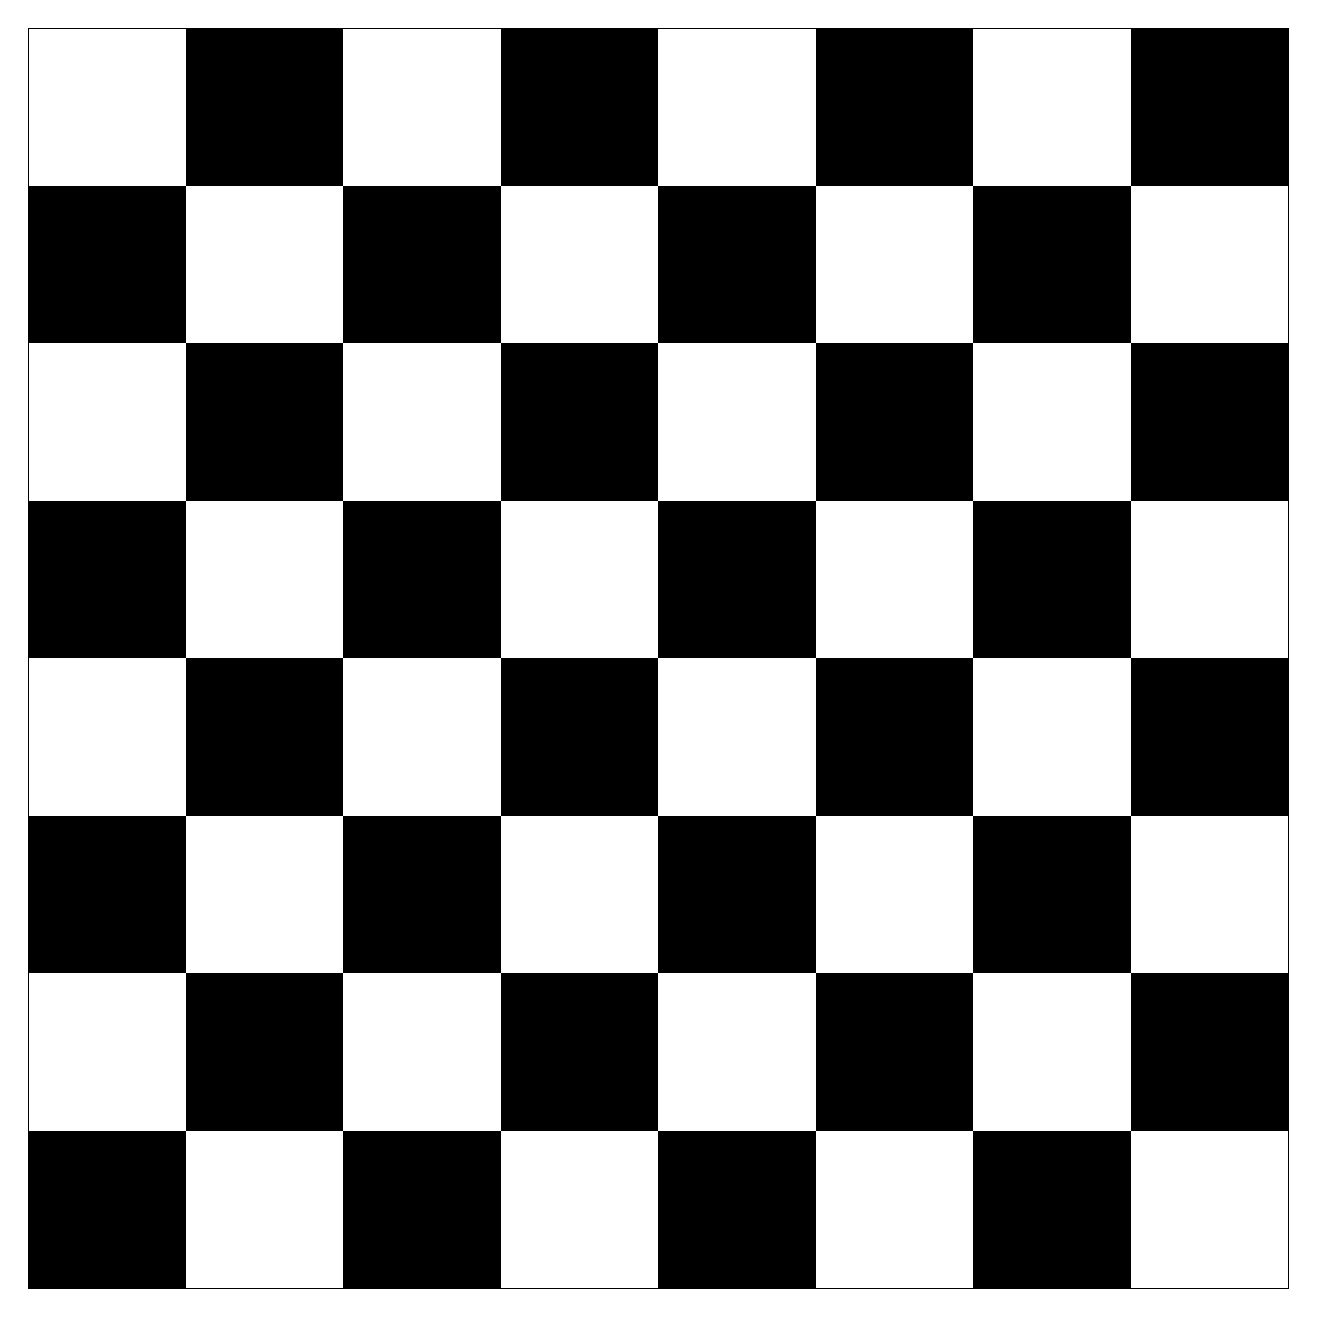
\begin{tikzpicture}[scale=2]
    \foreach \i in {0,1,...,7} {
      \foreach \j in {0,1,...,7} {
        \pgfmathtruncatemacro{\shade}{mod(\i+\j,2)}
        \ifnum\shade=0
          \fill[black] (\i,\j) rectangle ++(1,1);
        \else
          \fill[white] (\i,\j) rectangle ++(1,1);
        \fi
      }
    }
    \draw (0,0) rectangle (8,8);
  \end{tikzpicture}


\newpage


\begin{tikzpicture}[scale=2]
  \foreach \i in {0,1,...,7} {
    \foreach \j in {0,2,...,6} {
    \pgfmathtruncatemacro{\shade}{mod(\i+\j,3)}
    \ifnum\shade=0
      \draw[fill=UGLiBlue!50] (\i,\j) rectangle ++(1,2);
    \else
    \ifnum\shade=1
    \draw[fill=UGLiRed!50] (\i,\j) rectangle ++(1,2);
    \else
    \draw[fill=UGLiGreen!50] (\i,\j) rectangle ++(1,2);
    \fi
    \fi
    }
    }
\end{tikzpicture}
\end{center}
\end{document}